% Template for ICASSP-2026 paper; to be used with:
%          spconf.sty  - ICASSP/ICIP LaTeX style file, and
%          IEEEbib.bst - IEEE bibliography style file.
% --------------------------------------------------------------------------
\documentclass{article}
\usepackage{spconf,amsmath,graphicx,hyperref}
\usepackage{amsfonts}
\usepackage{booktabs}
\usepackage{placeins}
\usepackage{balance}
% Example definitions.
% --------------------
\def\x{{\mathbf x}}
\def\L{{\cal L}}
\newtheorem{pro}{Proposition}
\newtheorem{them}{Theorem}
\newtheorem{prf}{Proof}
\newtheorem{rmk}{Remark}
% Title.
% ------
\title{SARC: Structured Analytic-Residual Correction for \\Lightweight Multichannel Speech Enhancement}
%
% Single address.
% ---------------
\name{Gurui Jin$^{\star}$\quad Xiao-Ping Zhang$^{\star}$\quad Le Xiao \quad Yue Wang
\thanks{This work was supported by Shenzhen Ubiquitous Data Enabling Key Lab under grant ZDSYS20220527171406015.  Part of this work was conducted during an industry internship under a confidentiality agreement.}
\thanks{The code is available at https://github.com/jgr2021/SARC.}
\thanks{ Corresponding author: Xiao-Ping Zhang.}
}
\address{$^{\star}$ Shenzhen Ubiquitous Data Enabling Key Lab, Shenzhen International Graduate School, Tsinghua University}

\begin{document}
%\ninept
%
\maketitle
%
\begin{abstract}
Analytic spatial filters preserve a calibrated target response but can leave interference which is difficult to identify from their output alone.
We propose Structured Analytic-Residual Correction (SARC), a lightweight framework that combines analytic spatial filtering with neural correction
for multichannel speech enhancement.
A learned channel-weighting matrix
first forms a unit-response analytic estimate from RTF-aligned microphone
signals. The key idea is to subtract this estimate from the aligned
channels, canceling the modeled target while retaining channel-to-channel
nuisance differences. These target-canceling residuals, together with the
analytic estimate and a residual scale, guide a compact neural corrector
to suppress the remaining interference.
On a fixed four-microphone evaluation set, the 46,834-parameter SARC achieves
$17.527$ dB SI-SDR improvement and $2.730$ PESQ.
\end{abstract}
%
\begin{keywords}
Multichannel speech enhancement, relative transfer function, neural beamforming, residual correction
\end{keywords}
%
\section{Introduction}
\label{sec:intro}

A compact microphone array captures desired speech and nonstationary
noise through multiple microphone paths. When a calibrated target
response is available, classical methods can exploit this spatial
structure explicitly. The generalized sidelobe canceller (GSC)
separates a constrained target path from adaptive
cancellation~\cite{griffiths1982gsc,hoshuyama1999robust}, the
speech-distortion-weighted multichannel Wiener filter (SDW-MWF)
controls target distortion~\cite{spriet2004sdwmwf}, and the
maximum-likelihood-based adaptive interference canceller (ML-AIC)
combines blocking with a time-varying Gaussian source
model~\cite{wang2023mlaic}. However, such model-based adaptation can
be restrictive under rapidly changing interference.

Neural systems learn spatial statistics~\cite{casebeer2021nice},
multichannel filters~\cite{li2022eabnet}, or direct spectral--spatial
mappings~\cite{yang2023mcnet}. An unconstrained direct mapping,
however, does not explicitly preserve the calibrated target response.
Recent hybrid approaches therefore combine learned modules with
explicit spatial structure. AFnet uses relative transfer function
(RTF)-supervised alignment~\cite{lee2025afnet}, while other methods
embed analytic beamforming or Wiener filtering between learned
modules~\cite{lee2024mvdrunet,hsieh2024nwf,cheong2025ideeppe}.
However, a post-neural-filter that receives only the analytic output cannot use
multichannel differences to identify residual interference.

In this paper, we propose Structured Analytic-Residual Correction
(SARC), a lightweight multichannel speech enhancement method that
retains these spatial differences for neural correction. A
pre-calibrated frontal RTF first aligns the microphone signals, and
learned channel weighting forms a unit-response analytic estimate
$z$. The key step constructs the spatial residual
$\mathbf r=\mathbf y-\mathbf1 z$, which cancels the modeled target
component. A compact neural corrector then uses $(z,\mathbf r,v)$ to estimate the
remaining interference and refine $z$.
With only 46,834 parameters,
SARC achieves $17.527\!\pm\!.053$~dB SI-SDR improvement, exceeding a
matched direct mapping (14.198~dB) and ML-AIC (13.403~dB).


\section{Problem Formulation}
\label{sec:problem}

We consider multichannel speech enhancement with a fixed,
pre-calibrated target relative transfer function (RTF).
Let
$\mathbf{x}_{ft}=[x_{1ft},\ldots,x_{Mft}]^T\in\mathbb{C}^M$
denote the array short-time Fourier transform (STFT) at frequency
bin $f$ and frame $t$. For an $M$-microphone array,
\begin{equation}
	\mathbf{x}_{ft}
	=
	\mathbf{a}_f s_{ft}
	+
	\mathbf{n}_{ft},
	\label{eq:obs}
\end{equation}
where $s_{ft}\in\mathbb{C}$ is the target image at the reference
microphone, $\mathbf{a}_f\in\mathbb{C}^M$ is the target RTF, and
$\mathbf{n}_{ft}$ contains all other components. We assume that
$\mathbf{a}_f$ is fixed and pre-calibrated, with
$a_{f,\mathrm{ref}}=1$. The goal is to estimate $s_{ft}$ from the
multichannel observation $\mathbf{x}_{ft}$.

Suppressing $(f,t)$ for clarity, we first canonicalize the
microphone signals using the known RTF:
\begin{equation}
	\mathbf{y}
	=
	D(\mathbf{a})^{-1}\mathbf{x}
	=
	\mathbf{1}s+\boldsymbol{\eta},
	\qquad
	\boldsymbol{\eta}
	=
	D(\mathbf{a})^{-1}\mathbf{n},
	\label{eq:canonical}
\end{equation}
where $D(\mathbf{a})$ places the RTF on its diagonal and
$\mathbf{1}\in\mathbb{C}^M$ is the all-one vector.
After canonicalization, the modeled target component is identical
across all aligned microphone channels.

Consider a spatial filter $\mathbf{q}$ satisfying the unit-response
constraint
\begin{equation}
	\mathbf{q}^H\mathbf{1}=1.
\end{equation}
Its output is
\begin{equation}
	z
	=
	\mathbf{q}^H\mathbf{y}
	=
	s+e,
	\qquad
	e
	=
	\mathbf{q}^H\boldsymbol{\eta},
	\label{eq:analytic_est}
\end{equation}
where $e$ denotes
the interference remaining in the analytic estimate.
The desired enhanced output can be written as
\begin{equation}
	\hat{s}
	=
	z+\delta,
	\qquad
	\delta
	\approx
	s-z
	=
	-e.
	\label{eq:correction}
\end{equation}
However, observing only $z=s+e$ provides limited information for
distinguishing the target from the residual interference. In contrast,
the aligned multichannel observation $\mathbf{y}$ still contains
channel-to-channel differences related to the nuisance components.
The remaining problem is therefore to construct an observable
multichannel reference from $\mathbf{y}$ and $z$ that exposes
information about $e$ and can guide the correction $\delta$.


\section{Structured Analytic-Residual Correction}
\label{sec:sarc}

Figure~\ref{fig:architecture} shows SARC: a precision network determines channel weights, a deterministic layer forms $(z,\mathbf r,v)$, and a correction network predicts an update to cancel the remaining interference.

\begin{figure*}[t]
\centering
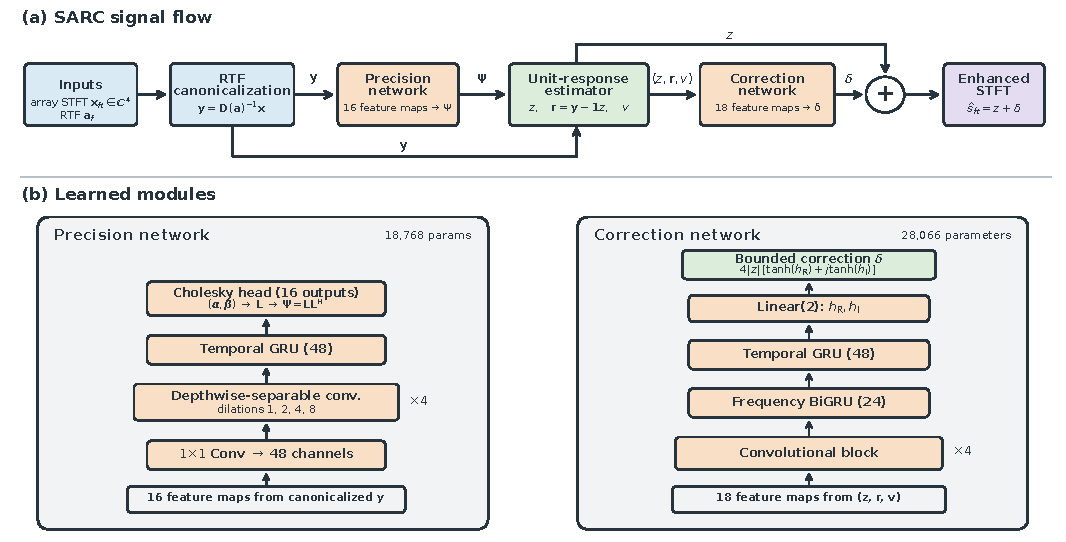
\includegraphics[width=.98\textwidth]{figures/sarc_architecture.pdf}
\caption{SARC architecture. Blue blocks denote observed inputs or fixed calibration operations, orange blocks are learned, green blocks are deterministic, and gray blocks construct features. The precision network outputs $\mathbf L$; the structured front end forms $\boldsymbol\Psi$, $z$, $v$, and $\mathbf r$. The residual exposes channel-to-channel nuisance differences for neural correction, while $z$ bypasses the corrector so that $\widehat s=z+\delta$.}
\label{fig:architecture}
\end{figure*}

\subsection{RTF canonicalization}

Equation~\eqref{eq:canonical} divides out the pre-calibrated frontal RTF, making the target response the fixed direction $\mathbf1$~\cite{kovalyov2023dfsnet,lee2025afnet}. No microphone coordinates are used; spatial responses enter through $\mathbf a_f$.

\subsection{Precision network and analytic estimate}

To infer relative channel reliability, we normalize $\mathbf y$ by its array root-mean-square (RMS) $\rho$. Each $u_m=y_m/\rho$ contributes real, imaginary, and log-magnitude feature maps~\cite{hu2020dccrn,rong2024gtcrn}; common phase, pairwise power balance, and normalized channel spread add four global feature maps, giving $3M+4=16$ inputs.

The analytic estimator requires a positive-definite weighting matrix for channel combination and residual measurement. Neural Cholesky parameterization has likewise been used to guarantee valid covariance estimates~\cite{deppisch2026mimo}. Here four time-causal convolutional blocks and a 48-unit forward GRU output the $M^2$ real degrees of freedom of a complex Cholesky factor:
\begin{equation}
\begin{aligned}
L_{mm}&=\exp(1.5\tanh\alpha_m),\\
L_{mk}&=.7(\tanh\beta^{\mathrm R}_{mk}+j\tanh\beta^{\mathrm I}_{mk}),\quad m>k.
\end{aligned}
\label{eq:cholesky}
\end{equation}
Here $\alpha_m$, $\beta^{\mathrm R}_{mk}$, and $\beta^{\mathrm I}_{mk}$ are real network outputs. For $M=4$, four positive diagonal and six complex lower-triangular entries require 16 real values. The learned nuisance weighting matrix $\boldsymbol\Psi=\mathbf L\mathbf L^{\mathrm H}\succ\mathbf0$ is positive definite by construction. A fixed MVDR-form unit-response estimator~\cite{tesch2021nonlinear} then computes
\begin{equation}
d=\mathbf1^{\mathrm H}\boldsymbol\Psi\mathbf1,\qquad
\mathbf q=\frac{\boldsymbol\Psi\mathbf1}{d},\qquad
z=\mathbf q^{\mathrm H}\mathbf y.
\label{eq:analytic}
\end{equation}
Because $\mathbf q^{\mathrm H}\mathbf1=1$, modeled target speech passes through $z$ unchanged; equivalently, $\mathbf w=\mathbf D(\mathbf a)^{-\mathrm H}\mathbf q$ satisfies $\mathbf w^{\mathrm H}\mathbf a=1$ in the microphone domain.

\subsection{Spatial residual as an interference reference}
Using~\eqref{eq:analytic_error}, the deterministic layer forms
\begin{equation}
\mathbf r=\mathbf y-\mathbf1z=\boldsymbol\eta-\mathbf1e,
\qquad
\mathbf q^{\mathrm H}\mathbf r=0.
\label{eq:spatial_residual}
\end{equation}
The modeled target cancels in $\mathbf r$, leaving spatial nuisance references for estimating $e$, as in GSC and ML-AIC blocking paths~\cite{griffiths1982gsc,wang2023mlaic}. The raw pair also reconstructs $\mathbf y=\mathbf1z+\mathbf r$ before feature normalization; this is an auxiliary structural property.

The corrector also needs a scale for the plausible error of $z$. We define the scale proxy
\begin{equation}
v=\frac{\mathbf r^{\mathrm H}\boldsymbol\Psi\mathbf r}
{(M-1)d}
\label{eq:scale}
\end{equation}
It converts precision-weighted disagreement to the scale of $z$. The quantity $v$ summarizes residual energy to condition the corrector.

\subsection{Correction network}

The corrector receives six bounded feature maps describing the magnitude and phase of $z$ and the absolute and relative scales of $v$. Each RMS-normalized residual channel contributes real, imaginary, and log-magnitude feature maps, giving $6+3M=18$ inputs. Thus $z$ supplies the current speech estimate, $\mathbf r$ supplies spatial interference references, and $v$ supplies a conditioning scale.

After four causal convolutional blocks, a 24-unit bidirectional frequency GRU and a 48-unit forward temporal GRU follow the frequency--time factorization of dual-path enhancement models~\cite{rong2024gtcrn}. They output two real coordinates $h_{\mathrm R}$ and $h_{\mathrm I}$ for Cartesian complex prediction~\cite{hu2020dccrn}. The bounded correction is
\begin{equation}
\begin{aligned}
\delta&=C|z|\,[\tanh(h_{\mathrm R})+j\tanh(h_{\mathrm I})],\quad C=4,\\
\widehat s&=z+\delta.
\end{aligned}
\label{eq:correction}
\end{equation}
Here $|z|$ supplies the local STFT amplitude scale, while $\tanh(\cdot)$ bounds each Cartesian update by $C|z|$; $v$ conditions the network but does not scale its output. The supervised update $s-z=-e$ trains the corrector to cancel the interference in $z$. The precision and correction networks contain 18,768 and 28,066 parameters, respectively.

\subsection{Training objective}
\label{sec:training}

Let $S=[s_{ft}]$ and $\widehat S=[\widehat s_{ft}]$ be the target and predicted STFTs, $s_{\mathrm{wav}}$ the clean waveform, and $\langle\cdot\rangle$ the mean over valid bins and examples. With power-law compression $c(X)=|X|^{0.3}e^{j\angle X}$~\cite{braun2021losses}, we combine spectral error and SI-SDR~\cite{leroux2019sisdr}:
\begin{align}
\mathcal L_C(X)&=\frac{\langle|c(X)-c(S)|^2\rangle}
{\langle|c(S)|^2\rangle},\nonumber\\
\mathcal L_{\mathrm{SI}}(X)&=-\frac1{20}\operatorname{SI\mbox{-}SDR}
(\operatorname{iSTFT}(X),s_{\mathrm{wav}}),\nonumber\\
\mathcal L_{\mathrm{enh}}(X;\lambda)&=\mathcal L_C(X)+
\lambda\mathcal L_{\mathrm{SI}}(X).
\label{eq:signal_losses}
\end{align}

During training, normalize the known nuisance $\boldsymbol\eta=\mathbf y-\mathbf1S$ as $\widetilde{\boldsymbol\eta}=\boldsymbol\eta/(M^{-1}\sum_m|\eta_m|^2)^{1/2}$. Motivated by the quadratic and log-determinant terms of Gaussian precision fitting~\cite{PRML}, we introduce the regularizer
\begin{equation}
\mathcal L_{\mathrm{prec}}=\left\langle
\frac{\widetilde{\boldsymbol\eta}^{\mathrm H}\boldsymbol\Psi
\widetilde{\boldsymbol\eta}-\log\det\boldsymbol\Psi}{M}
\right\rangle
\label{eq:precision_loss}
\end{equation}
to fit relative nuisance structure and fix the scale of $\boldsymbol\Psi$ without asserting an exact inverse covariance. Let $\bar p_s=F^{-1}\sum_f|S_{ft}|^2$. The auxiliary losses are
\begin{align}
\mathcal L_{\mathrm{corr}}&=\left\langle\frac{|\delta-(S-z)|^2}
{v+10^{-3}\bar p_s}\right\rangle,\nonumber\\
\mathcal L_{\mathrm{size}}&=\left\langle\frac{|\delta|^2}
{|z|^2+v}\right\rangle,\nonumber\\
\mathcal L_{\mathrm{sc}}&=\left\langle\frac{|z-S|^2}{v}
+\log\frac{v}{\bar p_s}\right\rangle.
\label{eq:auxiliary_losses}
\end{align}
Motivated by staged alignment/filter optimization~\cite{lee2025afnet}, SARC first trains the analytic estimator, then the corrector with the precision network frozen, and finally both modules jointly:
\begin{align}
\mathcal L_{\mathrm{sp}}&=\mathcal L_{\mathrm{enh}}(z;.10)
+.02\mathcal L_{\mathrm{prec}}+.001\langle\|\mathbf q\|_2^2\rangle,\nonumber\\
\mathcal L_{\mathrm{net}}&=\mathcal L_{\mathrm{enh}}(\widehat S;.12)
+.03\mathcal L_{\mathrm{corr}}+.001\mathcal L_{\mathrm{size}},\nonumber\\
\mathcal L_{\mathrm{joint}}&=\mathcal L_{\mathrm{net}}+.10\mathcal L_C(z)
+.02\mathcal L_{\mathrm{prec}}+.01\mathcal L_{\mathrm{sc}}.
\label{eq:stage_objectives}
\end{align}

\section{Experiments}
\begin{table*}[t]
\centering
\caption{Comparison on the fixed four-microphone evaluation set. Learned quality scores report mean $\pm$ sample standard deviation over three runs. Runtimes are medians for a 4-s input (Sec.~\ref{sec:comparison}); dashes denote no timing test.}
\label{tab:main}
\setlength{\tabcolsep}{3.8pt}
\resizebox{0.98\textwidth}{!}{%
\begin{tabular}{lcrrrrrr}
\toprule
System & Mics & GPU (ms) & CPU (ms) & Parameters & $\Delta$SI-SDR (dB) & STOI & PESQ\\
\midrule
Input microphone & 1 & --- & --- & 0 & 0 & .766 & 1.237\\
Norm-constrained GSC~\cite{hoshuyama1999robust} & 4 & --- & \textbf{174.0} & 0 & 7.854 & .922 & 1.583\\
Online SDW-MWF~\cite{spriet2004sdwmwf} & 4 & --- & 348.9 & 0 & 8.138 & .874 & 1.593\\
ML-AIC~\cite{wang2023mlaic} & 4 & --- & 209.6 & 0 & 13.403 & \textbf{.988} & 2.288\\
Online McNet~\cite{yang2023mcnet} & 4 & 170.0 & 2,831.5 & 1,837,250 & $11.355\!\pm\!.700$ & $.915\!\pm\!.008$ & $2.263\!\pm\!.071$\\
AFnet~\cite{lee2025afnet} & 4 & 74.6 & 1,459.0 & 2,554,896 & $10.102\!\pm\!.018$ & $.923\!\pm\!.005$ & $2.257\!\pm\!.059$\\
EaBNet~\cite{li2022eabnet} & 4 & 37.3 & 701.6 & 2,825,160 & $12.105\!\pm\!.133$ & $.933\!\pm\!.001$ & $2.142\!\pm\!.062$\\
\textbf{SARC} & 4 & \textbf{28.0} & 458.7 & 46,834 & $\mathbf{17.527\!\pm\!.053}$ & $.961\!\pm\!.001$ & $\mathbf{2.730\!\pm\!.057}$\\
\bottomrule
\end{tabular}}
\end{table*}

\subsection{Experimental setup}
All systems use the same four microphone channels at 16~kHz, with the first selected channel as reference. The fixed evaluation set has 80 mixtures from 20 unseen LibriSpeech speakers~\cite{panayotov2015librispeech}, balanced over four evaluation conditions and five SNRs from $-10$ to 10~dB, with one or two source-disjoint ESC-50 interferers~\cite{piczak2015esc50}. The spatial transfer functions are shared across compared systems. Training, validation, and test crops use disjoint time intervals.

RTF-dependent methods receive the same fixed frontal calibration, and all neural baselines receive the same four signals. SARC uses a 512-point STFT, a 25-ms square-root Hann window, and a 10-ms hop. We report $\Delta$SI-SDR, STOI~\cite{taal2011stoi}, and wideband PESQ~\cite{itu2005pesqwb}. Learned systems report mean and sample standard deviation over three runs.

GSC, SDW-MWF, and ML-AIC follow their published algorithms. McNet uses author code and an adapted checkpoint, EaBNet uses the official architecture trained locally, and AFnet is reimplemented from its paper. Outputs are rescored on identical trials. Paired 95\% confidence intervals use 30,000-draw cluster bootstraps over seed, speaker, and evaluation condition.

\subsection{Comparison with existing systems}
\label{sec:comparison}
SARC obtains the highest mean $\Delta$SI-SDR and PESQ. Against ML-AIC, it improves SI-SDR by 4.125~dB (95\% CI: 2.109--5.941~dB) and PESQ by .441 (95\% CI: .208--.643). ML-AIC has the highest STOI (.988 versus .961), with a .0267 advantage (95\% CI: .0142--.0433). Among the neural baselines, EaBNet gives the highest $\Delta$SI-SDR at 12.105~dB; SARC exceeds it by 5.423~dB (95\% CI: 3.630--6.959~dB).

Figure~\ref{fig:stft_example} shows a 0-dB example selected near the median SARC improvement in this SNR group. SARC suppresses background energy while retaining visible harmonic structure.

\begin{figure}[!htb]
\centering
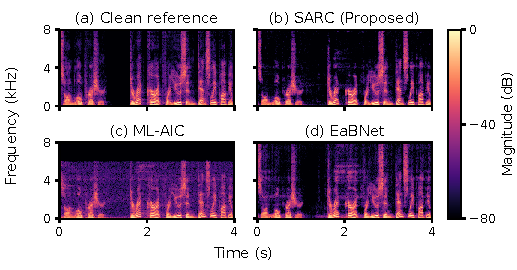
\includegraphics[width=\columnwidth]{figures/sarc_stft_example.pdf}
\caption{Synchronized clean reference and enhanced STFT magnitudes, with a shared color scale and no per-signal normalization.}
\label{fig:stft_example}
\end{figure}

Table~\ref{tab:main} reports full-utterance times on an RTX~4060 laptop GPU and single-thread i7-13650HX CPU, including STFT/iSTFT but excluding I/O and device transfers. Neural timings pool two rounds of 10 runs with reversed method order and 3 warmups per round (seed 1, batch 1, PyTorch~2.5.1, FP32). Classical timings retain 10 runs from a separate session (MATLAB~R2024b, FP64).

In this benchmark, SARC is 1.3--6.1 times faster on GPU and 1.5--6.2 times faster on CPU than the neural baselines. Classical implementations show lower CPU times, although cross-family comparisons involve different sessions, software, and precision.

\subsection{Ablation study}
\label{sec:ablation}
\begin{table}[t]
\centering
\caption{Ablations of the SARC mechanism on the same evaluation set.}
\label{tab:ablation}
\setlength{\tabcolsep}{3.2pt}
\resizebox{\columnwidth}{!}{%
\begin{tabular}{lrl}
\toprule
Configuration & $\Delta$SI-SDR (dB) & Component examined\\
\midrule
Analytic $z$ only & $11.333\!\pm\!.276$ & Without correction network\\
Identity precision + correction & $13.798\!\pm\!.230$ & Without channel weighting\\
Direct mapping & $14.198\!\pm\!.543$ & Without analytic structure\\
ML-AIC + same correction & $15.301\!\pm\!.749$ & Different analytic front-end\\
\textbf{SARC} & $\mathbf{17.527\!\pm\!.053}$ & Proposed method\\
\bottomrule
\end{tabular}}
\end{table}

Table~\ref{tab:ablation} supports four design choices: correction improves the analytic estimate; learned channel weighting improves on identity precision; analytic structure outperforms capacity-matched direct mapping; and SARC's front end performs better than ML-AIC with the same correction topology. These controls support the combined design, but do not isolate residual-input benefits.

\section{Conclusion}

SARC uses target-canceling spatial residuals to guide a bounded neural correction of interference remaining in a unit-response analytic estimate. On the fixed four-microphone evaluation set, the 46,834-parameter model achieves $17.527\!\pm\!.053$~dB SI-SDR improvement and $2.730\!\pm\!.057$ PESQ, exceeding the matched direct mapping and ML-AIC in these metrics; ML-AIC retains the highest STOI. The results support combining calibrated spatial estimation with residual-guided correction.

\clearpage

\balance
\bibliographystyle{IEEEbib}
\bibliography{strings,refs,sarc_refs}

\end{document}
